% !TEX TS-program = pdflatex
% !TEX encoding = UTF-8 Unicode

% This is a simple template for a LaTeX document using the "article" class.
% See "book", "report", "letter" for other types of document.

\documentclass[11pt]{article} % use larger type; default would be 10pt

\usepackage[utf8]{inputenc} % set input encoding (not needed with XeLaTeX)

%%% Examples of Article customizations
% These packages are optional, depending whether you want the features they provide.
% See the LaTeX Companion or other references for full information.

%%% PAGE DIMENSIONS
\usepackage{geometry} % to change the page dimensions
\geometry{a4paper} % or letterpaper (US) or a5paper or....
% \geometry{margin=2in} % for example, change the margins to 2 inches all round
% \geometry{landscape} % set up the page for landscape
%   read geometry.pdf for detailed page layout information

\usepackage{graphicx} % support the \includegraphics command and options

% \usepackage[parfill]{parskip} % Activate to begin paragraphs with an empty line rather than an indent

%%% PACKAGES
\usepackage{booktabs} % for much better looking tables
\usepackage{array} % for better arrays (eg matrices) in maths
\usepackage{paralist} % very flexible & customisable lists (eg. enumerate/itemize, etc.)
\usepackage{verbatim} % adds environment for commenting out blocks of text & for better verbatim
\usepackage{subfig} % make it possible to include more than one captioned figure/table in a single float
\usepackage{listings} % used to write pieces of code
\usepackage{xcolor}
% These packages are all incorporated in the memoir class to one degree or another...

%%% HEADERS & FOOTERS
\usepackage{fancyhdr} % This should be set AFTER setting up the page geometry
\pagestyle{fancy} % options: empty , plain , fancy
\renewcommand{\headrulewidth}{0pt} % customise the layout...
\lhead{}\chead{}\rhead{}
\lfoot{}\cfoot{\thepage}\rfoot{}

%%% SECTION TITLE APPEARANCE
\usepackage{sectsty}
\allsectionsfont{\sffamily\mdseries\upshape} % (See the fntguide.pdf for font help)
% (This matches ConTeXt defaults)

%%% ToC (table of contents) APPEARANCE
\usepackage[nottoc,notlof,notlot]{tocbibind} % Put the bibliography in the ToC
\usepackage[titles,subfigure]{tocloft} % Alter the style of the Table of Contents
\renewcommand{\cftsecfont}{\rmfamily\mdseries\upshape}
\renewcommand{\cftsecpagefont}{\rmfamily\mdseries\upshape} % No bold!

%%% END Article customizations

%%% The "real" document content comes below...

\title{Prova Finale - Reti Logiche (prof. William Fornaciari)}
\author{Corigliano Emilio 10627041 - 907936}
\date{A.A. 2020/21} % Activate to display a given date or no date (if empty)

\begin{document}
\maketitle

\section{Introduzione e spiegazione del problema}
Il progetto consiste nella progettazione di un circuito per l'equalizzazione di immagini in scala di grigi a 256 valori mediante il linguaggio di definizione hardware VHDL, attraverso il software \textit{Vivado}. L'equalizzazione è un processo di elaborazione digitale che consiste nell'elaborare l'immagine affinchè i suoi colori coprano tutto lo spettro disponibile. Nel nostro caso, dopo l'elaborazione vogliamo ottenere delle immagini che abbiano pixel di valore 0 e 255 rispettivamente nei punti di valore minimo e massimo nell'immagine originale; tutti gli altri pixel verranno ridistribuiti su tutto lo spettro in maniera coerente.

\begin{figure}[ht!]
\centering
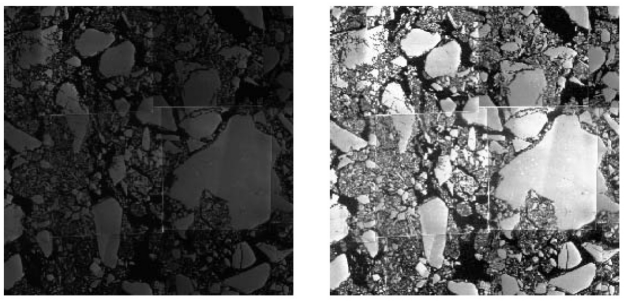
\includegraphics[width=120mm]{esempio-di-equalizzazione.png}
\caption{esempio di equalizzazione di un'immagine}
\end{figure}

\section{Considerazioni e scelte implementative}

\begin{itemize}
\item Non è necessario distinguere le varie righe, si può trattare la memoria semplicemente come un vettore di dimensione $N = R \cdot C$ da analizzare sequenzialmente
% una volta trovati i byte di valore massimo ($MAX\_PV$) e minimo ($MIN\_PV$)

\item Ogni byte in input all'indirizzo $mem[2+i]$ dovrà essere processato e l'output dovrà essere scritto in memoria all'indirizzo $mem[2+ N +i]$, con $i \in [0, N)$
\end{itemize}

\subsection{Fasi}
Ci sono 4 fasi fondamentali che occorre attraversare per elaborare l'immagine, ognuna delle quali ha bisogno di dati elaborati precedentemente. Per questo non sono ulteriormente parallelizzabili.

Si è scelto di affrontare ogni fase singolarmente per semplificare l'esposizione; questo approccio ha semplificato anche l'implementazione, di conseguenza le diverse fasi sono indipendenti tra loro. Seguendo questo approccio, però, si è limitata l'ottimizzazione della progettazione, facendo sì che alcuni componenti (come per esempio i contatori) non fossero in quantità minima ma sono stati replicati, in maniera leggermente diversa, per ogni fase in cui erano necessari. Questo però non è stato ritenuto un problema data la dimensione del progetto e la qualità dell'hardware per il quale è stato progettato; si è preferita la qualità e semplicità espositiva alla ottimizzazione progettuale.

\begin{figure}[ht!]
\centering
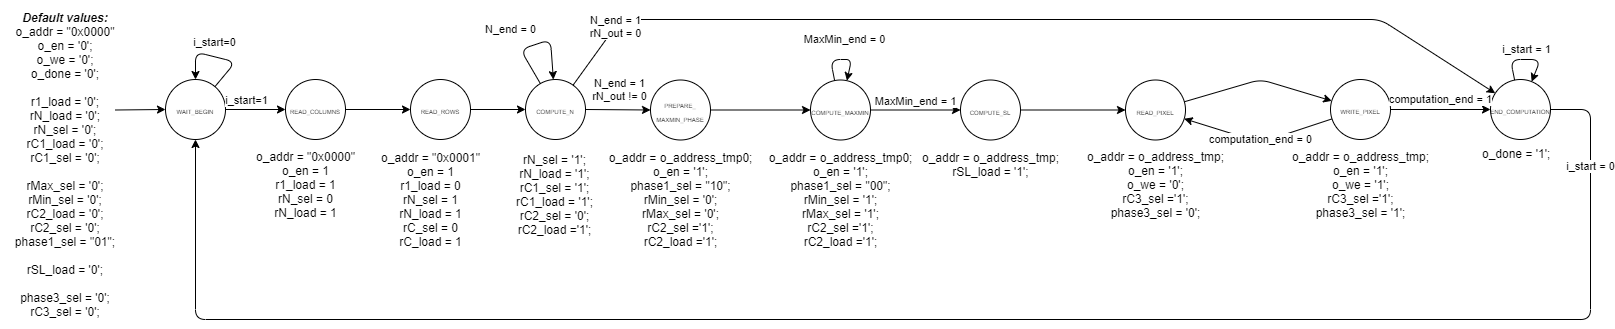
\includegraphics[width=150mm]{datapaths/FSM.png}
\caption{FSM dell'elaborazione}
\end{figure}

\subsubsection{computazione della quantità di pixel}
La prima fase è quella in cui si calcola la dimensione dell'immagine $N$ da equalizzare. Questo valore è ottenuto moltiplicando $mem[0]$ e $mem[1]$ tramite un moltiplicatore per somme successive. Alla fine dell'operazione viene portato in alto il segnale $N_end$ che indica la fine dell'operazione. Da questo momento fino alla prossima esecuzione nel registro $rN$ ci sarà il valore $N = R \cdot C$.

\begin{figure}[ht!]
\centering
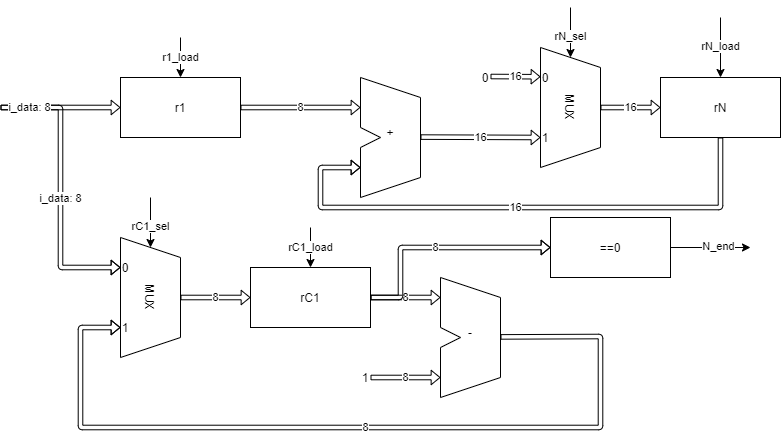
\includegraphics[width=120mm]{datapaths/regN.png}
\caption{computazione della quantità di pixel}
\end{figure}


\subsubsection{Ricerca dei valori massimi e minimi dei pixel}
Nella seconda fase si cercano il valore massimo ($MAX\_PV$) e il valore minimo ($MIN\_PV$): si scorre una prima volta tutta l'immagine e si cercano contemporaneamente il valore massimo e minimo dei pixel presenti nell'immagine. Per tenere conto dei pixel letti e per generare l'indirizzo al quale leggere il valore si usa un contatore che parte da 0 e ad ogni ciclo di clock incrementa di 1, fino a raggiungere $N$; a questo punto verrà portato in alto il segnale di $MaxMin_end$.

\begin{figure}[ht!]
\centering
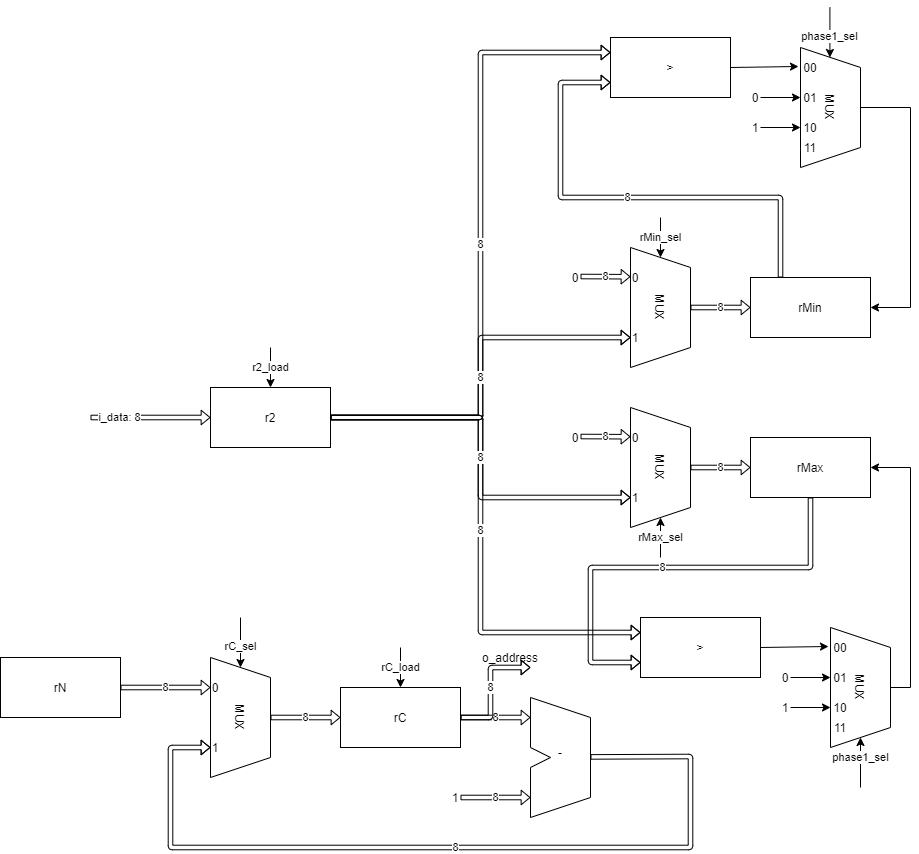
\includegraphics[width=120mm]{datapaths/regMax_regMin.png}
\caption{Ricerca dei valori massimi e minimi dei pixel}
\end{figure}


\subsubsection{Computazione del valore SHIFT\_LEVEL}
La terza fase prevede il calcolo dello $SHIFT\_LEVEL$; questo viene ottenuto implementando una funzione combinatoria (nell'immagine rappresentata con il blocco $f(x)$ avente come input 8 bit e come output 4 bit). La funzione combinatoria prende in input $MAX\_PV - MIN\_PV + 1$ (quindi il $DELTA\_VALUE$ incrementato di 1) perchè si era pensato che sarebbe stato più semplice la generalizzazione, per non avere le varie soglie fisse. Infatt

	\begin{lstlisting}[language=Python, caption=Generazione di soglie]
for i in range(256):
	print(str(i) + ": " + str(8 - math.floor(math.log2(i+1))))
	\end{lstlisting}

\begin{figure}[ht!]
\centering
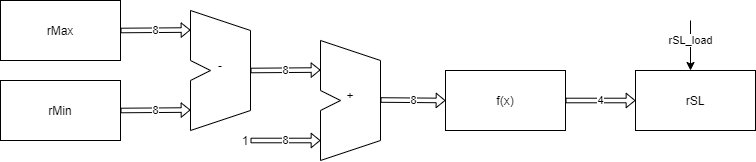
\includegraphics[width=120mm]{datapaths/regSL_final.png}
\caption{Ricerca dei valori massimi e minimi dei pixel}
\end{figure}


\subsubsection{Equalizzazione}
La quarta fase, quella finale, provvede a equalizzare l'immagine tramite l'algoritmo fornitoci. Per ogni pixel che compone l'immagine (scorsi grazie ad un contatore che parte da $N-1$ e decrementa fino a 0) si legge il valore originale. Al ciclo successivo si provvede a scrivere in memoria il valore computato all'indirizzo del pixel originale incrementato di $N$. Sono necessari due cicli per ogni pixel da equalizzare poichè la memoria prevede un solo segnale per codificare l'indirizzo su cui leggere o scrivere; visto che l'immagine originale non va sovrascritta si deve alternare una fase di lettura con una di scrittura.

\begin{figure}[ht!]
\centering
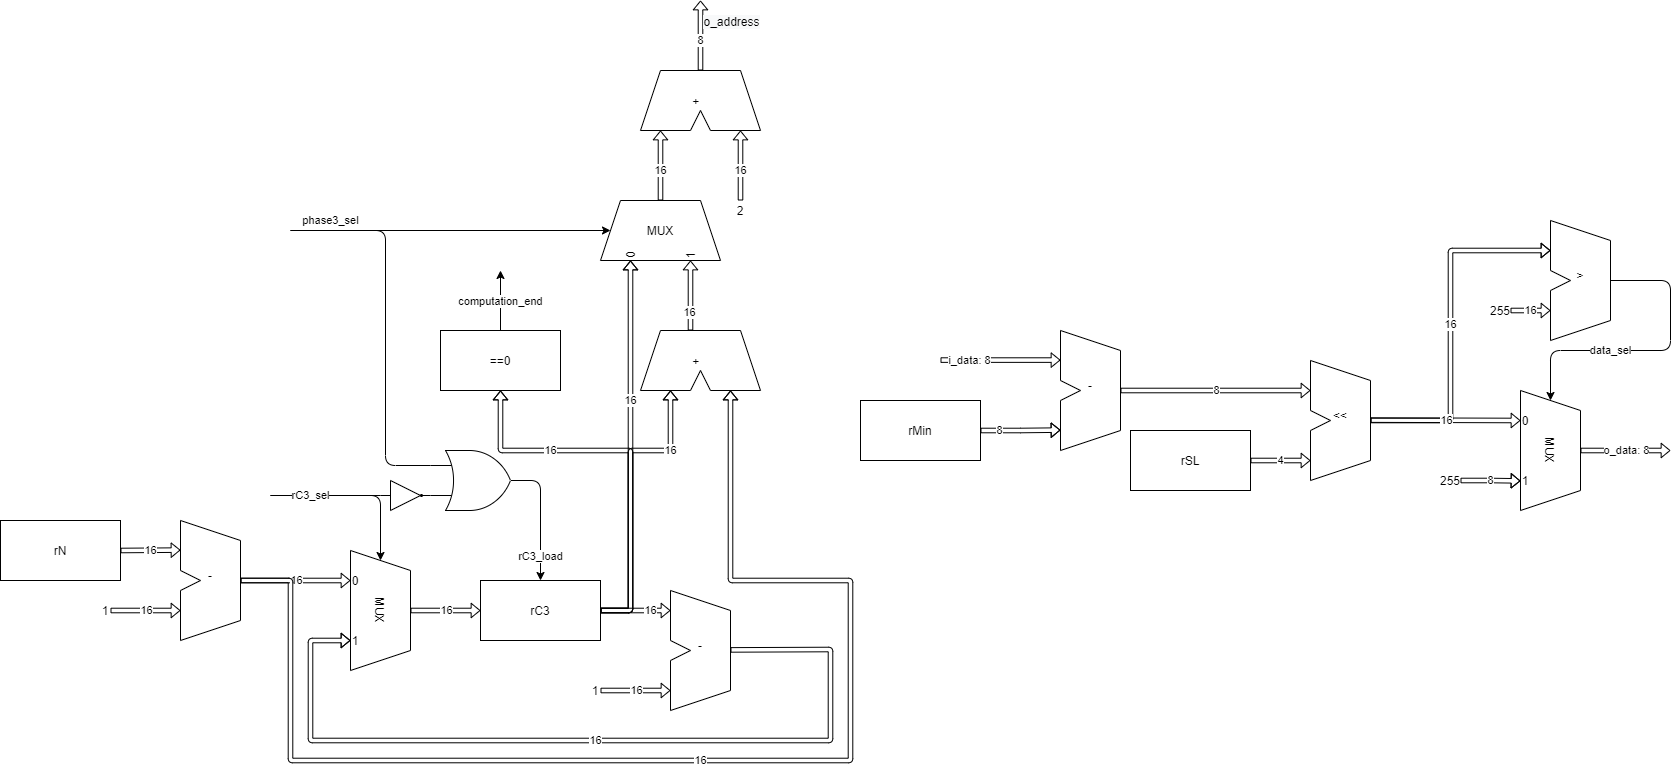
\includegraphics[width=120mm]{datapaths/computation.png}
\caption{Ricerca dei valori massimi e minimi dei pixel}
\end{figure}

\begin{itemize}
\item una quarta fase che è la vera e propria elaborazione dell'immagine, nella quale si scorre pixel per pixel, elaborandolo e scrivendolo nella regione di output della memoria (input: $mem[2+i]$; output: $mem[2+N+i]$)
\end{itemize}
 
\subsection{Registri}
\begin{itemize}
\item $RegN$: memorizza il numero totale di byte che compongono l'immagine
\item $RegMaxPL$: memorizza il livello massimo dei pixel presente nell'immagine
\item $RegMinPL$: memorizza il livello minimo dei pixel presente nell'immagine	
\item $RegShiftLevel$: memorizza lo $SHIFT\_LEVEL$, può essere computato a soglie dato che il delta value è l'unica variabile.
\item un contatore caricabile con un valore variabile che permetta di eseguire la moltiplicazione iniziale o che possa scorrere per tutto il vettore l'immagine
\end{itemize}

\section{testing}
Corner cases testati:
\begin{itemize}
\item grossa immagine
\item zero righe
\item zero colonne
\item stesso valore in tutta l'immagine
\item più immagini consecutive
\end{itemize}


\end{document}
